%! Suppress = MissingImport
%%
%% sample document for AAMAS'19 conference
%%
%% modified from sample-sigconf.tex
%%
%% see ACM instructions acmguide.pdf
%%
%% AAMAS-specific questions? F.A.Oliehoek@tudelft.nl
%%

\pdfminorversion=7  % Fixes .eps image files

\documentclass[sigconf]{aamas}  % do not change this line!
%% your usepackages here, for example:
\usepackage{booktabs}
\usepackage{listings}
\usepackage{graphicx}
\usepackage{float}
\usepackage{algorithm}
\usepackage{algorithmic}
\usepackage{appendix}
\usepackage{soul}
\usepackage{balance}
\usepackage[]{todonotes}

%% do not change the following lines
\setcopyright{ifaamas}  % do not change this line!
\acmDOI{doi}  % do noadat change this line!
\acmISBN{}  % do not change this line!
\acmConference[AAMAS'20]{Proc.\@ of the 19th International Conference on Autonomous Agents and Multiagent Systems
    (AAMAS 2020), B.~An, N.~Yorke-Smith, A.~El~Fallah~Seghrouchni, G.~Sukthankar (eds.)}{May 2020}{Auckland, New Zealand}  % do not change this line!
\acmYear{2020}  % do not change this line!
\copyrightyear{2020}  % do not change this line!
\acmPrice{}  % do not change this line!


%% the rest of your preamble here
\lstset{
    basicstyle=\ttfamily,
    columns=fullflexible,
    frame=single,
    breaklines=true,
    postbreak=\mbox{\textcolor{red}{$\hookrightarrow$}\space},
    basicstyle=\small,
}

%%%%%%%%%%%%%%%%%%%%%%%%%%%%%%%%%%%%%%%%%%%%%%%%%%%%%%%%%%%%%%%%%%%%%%%%%%%%%%%%%%%%%%%%%%%%%%%%%%%%%%%%%

\begin{document}

    \title{Auction-based Mechanisms for Allocating Elastic Resources in Edge Clouds}
%\titlenote{Produces the permission block, and copyright information}

% AAMAS: as appropriate, uncomment one subtitle line; check the CFP
%\subtitle{Extended Abstract}
%\subtitle{Industrial Applications Track}
%\subtitle{Socially Interactive Agents Track}
%\subtitle{Blue Sky Ideas Track}
%\subtitle{Engineering Multiagent Systems Track}
%\subtitle{Robotics Track}
%\subtitle{JAAMAS Track}
%\subtitle{Doctoral Mentoring Program}

%\subtitlenote{The full version of the author's guide is available as \texttt{acmart.pdf} document}


% AAMAS: submissions are anonymous for most tracks
    \author{Paper \#1263}  % put your paper number here!

%% example of author block for camera ready version of accepted papers: don't use for anonymous submissions
%

    \begin{abstract}  % put your abstract here!
        Edge cloud computing enables computational task to be process at the edge of the network using limited
        computational resource in comparison to larger remote data centres. Because of this, resource allocation and
        management is significantly more important. Existing resource allocations approaches usually assumed that tasks
        have inelastic resource requirements (i.e., a fixed amount of bandwidth and computation requirements) however
        this may result in inefficient resource usage due to unbalanced requirements from tasks resulting in resource
        bottlenecks. To address this, we propose a novel approach that takes advantage of the elastic nature of
        resource as time taken for an operation to occur is proportional to the resource allocated. This however make
        previous research incompatible with this problem. Therefore we describe this problem formally, show that it is
        NP-Hard and propose a scalable approximation algorithm. To deal with self-interested user, we demonstrate a
        centralised auction mechanism that is incentive compatible using the approximation algorithm. Moreover, we
        propose a novel decentralised iterative auction mechanism that doesn't require users to reveal their private
        task value but is not incentive compatible. In extensive simulations, we show that considering the elasticity
        of resources leads to a gain in utility of around 20\% compared to existing approaches with the proposed
        approaches typically achieving 95\% of the theoretical optimal.
    \end{abstract}


% AAMAS: the ACM CCS are not needed within AAMAS papers
%%
%% The code below should be generated by the tool at
%% http://dl.acm.org/ccs.cfm
%% Please copy and paste the code instead of the example below.
%%
%\begin{CCSXML}
%<ccs2012>
% <concept>
%  <concept_id>10010520.10010553.10010562</concept_id>
%  <concept_desc>Computer systems organization~Embedded systems</concept_desc>
%  <concept_significance>500</concept_significance>
% </concept>
% <concept>
%  <concept_id>10010520.10010575.10010755</concept_id>
%  <concept_desc>Computer systems organization~Redundancy</concept_desc>
%  <concept_significance>300</concept_significance>
% </concept>
% <concept>
%  <concept_id>10010520.10010553.10010554</concept_id>
%  <concept_desc>Computer systems organization~Robotics</concept_desc>
%  <concept_significance>100</concept_significance>
% </concept>
% <concept>
%  <concept_id>10003033.10003083.10003095</concept_id>
%  <concept_desc>Networks~Network reliability</concept_desc>
%  <concept_significance>100</concept_significance>
% </concept>
%</ccs2012>
%\end{CCSXML}
%
%\ccsdesc[500]{Computer systems organization~Embedded systems}
%\ccsdesc[300]{Computer systems organization~Redundancy}
%\ccsdesc{Computer systems organization~Robotics}
%\ccsdesc[100]{Networks~Network reliability}


    \keywords{Edge clouds; elastic resources; auctions}  % put your semicolon-separated keywords here!

    \maketitle

    %% start of main body of paper
    \section{Introduction}
\label{sec:introduction}
In the last few years, cloud computing~\cite{cloud_cite} has become a popular solution for running data-intensive
applications remotely. However, large-scale data centres are not feasible for application domains that require low
latency or high security and privacy. To deal with such domains, \emph{fog/edge computing}~\cite{mobile_edge_IoT} has
emerged as a complementary paradigm allowing tasks to be executed at the edge of networks, close to the user, in small
data centers, known as \emph{edge clouds}.

As the Internet-of-things grows, fog/edge cloud computing is a key enabling
technology~\cite{mobile_edge_IoT, edge_computing_iot}, in particular for applications
in smart cities~\cite{mobile_edge_smart}, disaster response scenarios~\cite{mobile_edge_disaster, smart_disaster_management},
home automation systems, etc. In these applications, low-powered devices
generate data or tasks that cannot be processed locally but are impractical to use with standard cloud computing
services. More specifically, in smart cities, these devices could be used to control smart traffic light
systems~\cite{smart_cities_traffic_lights} which collect data from roadside sensors to optimise the traffic light
sequence to minimise vehicle waiting times or to analyse video feeds from CCTV cameras~\cite{Sreenu2019}. In disaster
response~\cite{smart_disaster_management}, sensor data from autonomous vehicles can be aggregated to produce real-time
maps of devastated areas to help first responders better understand the situation and search for survivors.

To accomplish these tasks, there are typically several types of resources that are needed, including but not exclusively
communication bandwidth, computational power, and data storage resources~\cite{vaji_infocom}. These are tasks are
generally delay-sensitive, meaning the task may be finished as fast as possible or by a specific completion deadline. \\
When accomplished, different tasks carry different values for their owners often dependant on the importance of the
program tasks, e.g., analysing current levels of air pollution may be less important than preventing a large-scale
traffic jam at peak times or tracking a criminal on the run. \\
Given that edge clouds are often highly constrained in their resources~\cite{edge_limitations}, we are interested in
allocating tasks to edge cloud servers to maximize the overall social welfare achieved (i.e., the sum of completed task
values). This is particularly challenging, since users in edge clouds are typically self-interested and may behave
strategically~\cite{Bi2019} or may prefer not to reveal private information about their values to a central allocation
mechanism~\cite{Pai2013}.

An important shortcoming of existing work around resource allocation in edge cloud computing is that it assumes tasks
have strict resource requirements -- that is, each task must be allocated a fixed amount of CPU cycles or bandwidth by a
server. This is often achieved by users selecting a particular VM specification for their task, however, this can cause
both inefficient allocation of resources and bottlenecks on certain server resources when multiple tasks overrequest
particular resources.

Previous work~\cite{ServerElasticity} has considered the ability of cloud servers to flexibly respond to usage by
expanding resource capacity when needed. Due to the often ad hoc nature of fog cloud networks, such an ability is
generally not feasible, therefore in this work we utilise the ability for tasks to have flexibility in how its
resources are allocated due to the linear relationships of many task attributes.

An example is the time taken for a program to be download by the server is
generally proportional to the bandwidth allocated. This is similarly true for sending back of results to the users.
Computation is more difficult as the scalability of a program is dependant on the particular program, therefore this
work considers only tasks that are linearly scalability. We leaves for future work, the ability for task's to be
considered that scale non-linearly.

Using this capability to flexibly allocate resources is additionally important in the case of edge computing due to the
limited resources capacities that servers have in comparison to the large data centres used in standard cloud computing.
Therefore, using task resources flexibility, we propose a new resources allocation optimisation problem that enables
servers to have greater flexibility over how its resources are allocated. However, this new optimisation problem is
incompatible with previous research in this area, thus we propose three mechanisms that utilise this flexibility.

In the following section, an overview of related work is provided. Section~\ref{sec:problem-formulation} presents the
problem formulation, an optimisation problem, and an example case to show the effectiveness of such a system. Using this
formulation, Section~\ref{sec:flexible-resource-allocation-mechanisms} presents three different algorithms: a modular
greedy algorithm, a centralised incentive-compatible auction, and a novel decentralised iterative auction. Using these
algorithms, Section~\ref{sec:empirical-results} presents an extensive analysis of our mechanisms compared to the optimal
task, flexible solution and a strict resource requirement solution. .

    \section{Problem formulation}\label{sec:problem-formulation}
In this section we first describe the system model. Then, we present the optimization problem and prove its NP-hardness.
Final present an example problem to show the affect of the flexible resource allocation compared to fixed resource
allocation.

\begin{figure}[ht]
    \centering
    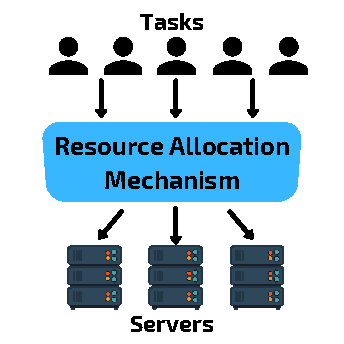
\includegraphics[width=0.6\linewidth]{figs/system_model.pdf}
    \caption{System Model}
    \label{fig:system_model}
\end{figure}

\subsection{System model}\label{subsec:system-model}
A sketch of the system is shown in Fig.~\ref{fig:system_model}.
We assume that in the system there is a set of servers $I = \{1,2,\ldots,\left|I\right|\}$ servers, which could be edge
clouds that can be accessed either through cellular base stations or WiFi access points (APs). These servers have
different types of limited resources: storage for the code/data needed to run a task (e.g., measured in GB),
computation capacity in terms of CPU cycles per time interval (e.g., measured in FLOP/s), and communication bandwidth
to receive the data and to send back the results of the task after execution (e.g., measured in Mbit/s). We assume
that the servers are heterogeneous in all their characteristics. More formally, we denote the storage capacity of
server $i$ with $S_i$, computation capacity with $W_i$, and the communication (bandwidth) capacity with $R_i$.

There is a set $J = \{1,2,\ldots,\left| J \right|\}$ of different tasks that require service from one of the servers.
\footnote{We focus on a single-shot setting in this paper. In practice, an allocation mechanism would repeat the
allocation decisions described here over regular time intervals, with longer-running tasks re-appearing on consecutive
time intervals. We leave a detailed study of this to future work.} Each task has a value, denoted $v_j$, representing
the value of running the task to its owner. To run any of these tasks on a server requires storing the appropriate
code/data on the same server. This storage size for the task $j$ is denoted as $s_j$ with the rate that the program
is transferred to the server as $s^{'}_j$. For a task to be computed successfully, it must fetch and execute
instructions on a CPU. We consider the total number of CPU cycles required for the program to be $w_j$, where the
number of CPU cycles are assigned to the task per unit of time as $w^{'}_j$. Finally, after the task is run and the
results obtained, the latter need to be sent back to the user. The size of the results for task $j$ is denoted with
$r_j$, and the bandwidth speed it is sent back to the user as $r^{'}_j$. Each task has a deadline, denoted by $d_j$,
as the maximum time for a task to be completed successfully. This time includes: the time required to send the
data/code to the server, run it on the server, and get back the results. We assume that there is an \emph{all} or
\emph{nothing} task execution reward scheme, meaning that the task value is awarded only if entire task loaded,
computed and the results sent back within the deadline.

\subsection{Optimization problem}\label{subsec:optimisation-problem}
Given the aforementioned assumptions from the system model, this requires two allocation mechanisms: the assignment of
tasks to servers and server resources to assigned task. This allocation mechanism is described by the following
optimisation where the variable $x_{i,j} \in \{0, 1\}$ describes if a task $j$ is running on server $i$.

\begin{align}
    \max & \sum_{\forall j \in J} v_j \left(\sum_{\forall i \in I} x_{i,j}\right)\label{eq:objective}\\
    \mbox{s.t.} \nonumber \\
    & \sum_{\forall j \in J} s_j x_{i,j} \leq S_i, &~ \forall i \in I,\label{eq:server_storage_constraint}\\
    & \sum_{\forall j \in J} w^{'}_j x_{i,j} \leq W_i, &~ \forall i \in I,\label{eq:server_computation_constraint}\\
    & \sum_{\forall j \in J} (r^{'}_j + s^{'}_j) \cdot x_{i,j} \leq R_i, &~ \forall i \in I,\label{eq:server_communication_constraint}\\
    & \frac{s_j}{s^{'}_j} + \frac{w_j}{w^{'}_j} + \frac{r_j}{r^{'}_j} \leq d_j, &~ \forall{j \in J},\label{eq:task_deadline}\\
    & 0 < s^{'}_j < \infty, &~ \forall{j \in J,}\label{eq:loading_speeds}\\
    & 0 < w^{'}_j < \infty, &~ \forall{j \in J,}\label{eq:compute_speeds}\\
    & 0 < r^{'}_j < \infty, &~ \forall{j \in J,}\label{eq:sending_speeds}\\
    & \sum_{\forall i \in I} x_{i,j} \leq 1, &~ \forall j \in J,\label{eq:server_task_allocation}\\
    & x_{i,j} \in \{0, 1\}, &~ \forall{i \in I},\forall{j \in J}.\label{eq:task_allocation}
\end{align}

The objective (Eq.\eqref{eq:objective}) is to maximize the total value over all tasks (i.e., the social welfare) that
are completed within the deadline (Eq.~\eqref{eq:task_deadline}. Constraints~\eqref{eq:server_storage_constraint},
~\eqref{eq:server_computation_constraint} and~\eqref{eq:server_communication_constraint} related to the finite resource
capacity of the servers, storage, computation and communication (bandwidth) respectively.
Constraint~\eqref{eq:server_storage_constraint} relates to the finite storage capacity for the task to store code/data
used to compute. With Eq.\eqref{eq:server_computation_constraint} being the finite computation capacity of each server.
The communication constraint (Eq.~\eqref{eq:server_communication_constraint}) comprises of two parts: the first for the
loading of the data/code onto the server, and the second for sending back the results to the user.
Constraint~\eqref{eq:task_deadline} forces the task to be completed within the task deadline, that being the sum of
time taken for all of the stages to complete in series (i.e.. loaded task onto server, computing the task, sending the
results back to the user). Note that if a task is not run on any server, this constraint can be satisfied by choosing
arbitrarily high bandwidth and CPU rates (as these resources do not use up any servers' resources in
Eq.~\eqref{eq:server_storage_constraint},~\eqref{eq:server_computation_constraint}
and~\eqref{eq:server_communication_constraint} when not allocated to server). The rates for each stage
($s^{'}_j$, $w^{'}_j$ and $r^{'}_j$) are all positive and finite (Eqs.~\eqref{eq:loading_speeds}
,~\eqref{eq:compute_speeds},~\eqref{eq:sending_speeds}). Further, every task is served by at most one server
(Eq.\eqref{eq:server_task_allocation}) as each task is either served or not by each server
(Eq.\eqref{eq:task_allocation}). \\


Using this optimisation problem, this is an extension of the knapsack problem that is well-studied and known to be
NP-hard with pseudo-polynomial time complexity using dynamic programming.
\begin{theorem}
    The optimisation problem as described in section~\ref{subsec:optimisation-problem} is NP-hard.
\end{theorem}
\begin{proof}
    The optimization problem without the constraint~\eqref{eq:task_deadline} is a 0--1 multidimensional knapsack
    problem~\cite{knapsackproblems_2004}, which is a generalization of a simple 0--1 knapsack problem. The latter is an
    NP-hard problem~\cite{knapsackproblems_2004}. Given this, it follows that the 0--1 multidimensional knapsack problem
    is also NP-hard. Since optimization problem (Eqs~\eqref{eq:objective} -~\eqref{eq:task_allocation}) is a
    generalization of a 0--1 multidimensional knapsack problem, it follows that it is NP-hard as well.
\end{proof}

\subsection{Example Problem Case}\label{subsec:example-problem-case}
Before we propose our novel allocation mechanisms for the allocation problem with elastic resources, we briefly
outline an example to illustrates why considering this elasticity is important. In this example, there are 12 potential
tasks and 3 servers (the exact settings can be found in table~\ref{table:example_tasks_properties} for the tasks and
table~\ref{table:example_servers_properties} for the servers). The figures~\ref{fig:fixed_resources_speeds}
and~\ref{fig:flexible_resources_speeds} represents each server as a group of three bars, each relating to the each
server's resource types, with the percentage of resources used by a task being the size of the bar.

\begin{figure}[th]
    \centering
    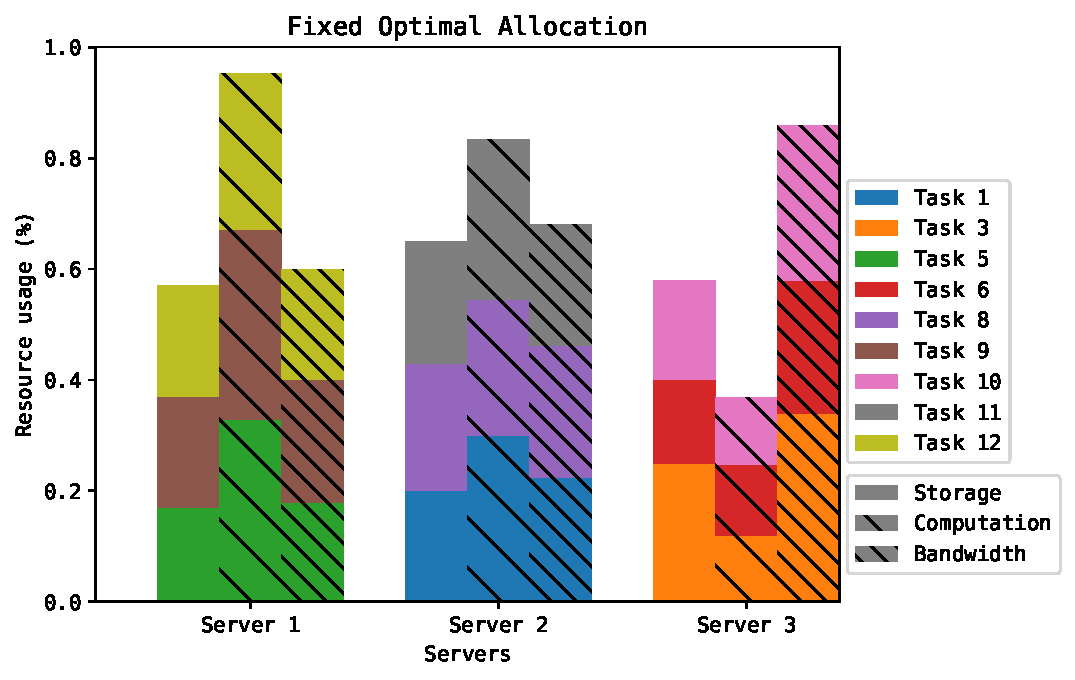
\includegraphics[width=\linewidth]{figs/allocation/fixed_optimal_allocation.pdf}
    \caption{Optimal solution with fixed resource speeds}
    \label{fig:fixed_resources_speeds}
\end{figure}

Figure~\ref{fig:fixed_resources_speeds} shows the best possible allocation if tasks have fixed resource speeds (that
were set by minimising the total amount of resources to be completed within the deadline). Here, only 9 of the tasks
are run, resulting in a total social welfare of 980 due to server 1 and 2's limited computational capacity and server
3' limited communication capacity.

\begin{figure}[th]
    \centering
    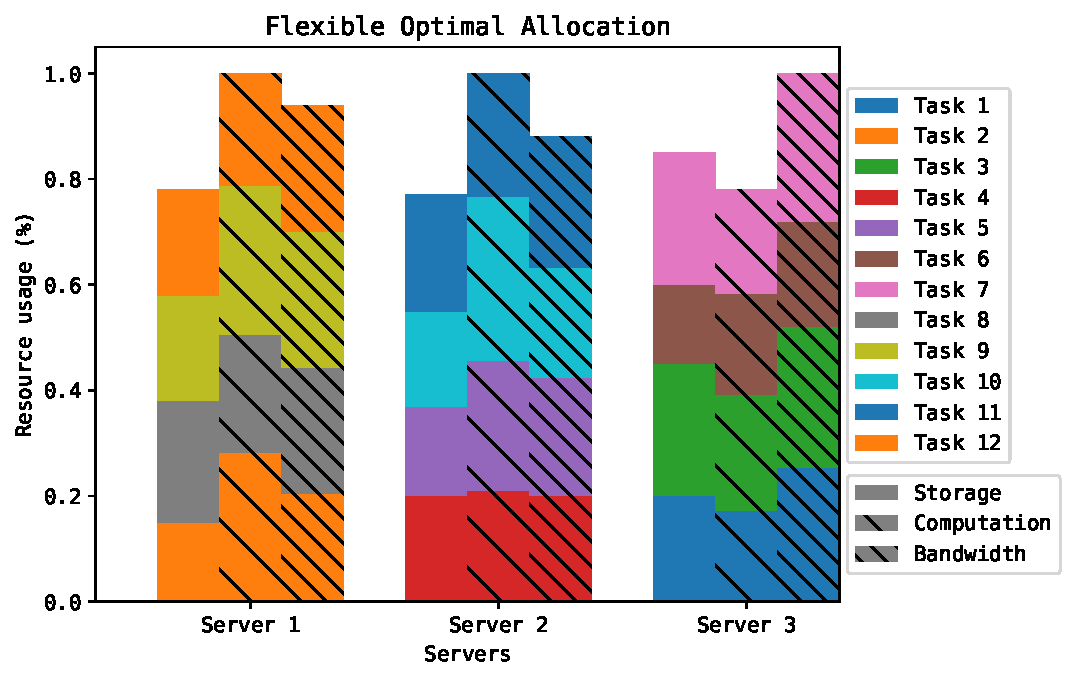
\includegraphics[width=\linewidth]{figs/allocation/flexible_optimal_allocation.pdf}
    \caption{Optimal solution with elastic resources. Compared to the fixed allocation, the elastic allocation is able
    to fully use all of its resources}
    \label{fig:flexible_resources_speeds}
\end{figure}

In contrast to figure~\ref{fig:fixed_resources_speeds}, Figure~\ref{fig:flexible_resources_speeds} depicts the optimal
allocation if elastic resources are considered. Here, all of the resources are used by the servers whereas the fixed
example~\ref{fig:fixed_resources_speeds} cant do this. In total, the elastic approach manages to schedule all 12 tasks
within the resource constraints, achieving a total social welfare of 1200 (an 18\% improvement over the fixed approach).

\begin{table}[h]
    \begin{tabular}{|c||c|c|c|}
        \hline
        Name & $S_i$ & $W_i$ & $R_i$ \\ [0.5ex] \hline\hline
        Server 1 & 400 & 100 & 220 \\ \hline
        Server 2 & 450 & 100 & 210 \\ \hline
        Server 3 & 375 & 90 & 250 \\ \hline
    \end{tabular}
    \caption{Table of server attributes}
    \label{table:example_servers_properties}
\end{table}

\begin{table}[h]
    \begin{tabular}{|c||c|c|c|c|c||c|c|c|}
        \hline
        Name & $v_j$ & $s_j$ & $w_j$ & $r_j$ & $d_j$ &  $s^{'}_j$ & $w^{'}_j$ & $r^{'}_j$ \\ [0.5ex] \hline\hline
        Task 1 & 100 & 100 & 100 & 50 & 10 & 30 & 27 & 17 \\ \hline
        Task 2 & 90 & 75 & 125 & 40 & 10 & 22 & 32 & 15 \\ \hline
        Task 3 & 110 & 125 & 110 & 45 & 10 & 34 & 30 & 17 \\ \hline
        Task 4 & 75 & 100 & 75 & 35 & 10 & 27 & 21 & 13 \\ \hline
        Task 5 & 125 & 85 & 90 & 55 & 10 & 24 & 28 & 17 \\ \hline
        Task 6 & 100 & 75 & 120 & 40 & 10 & 20 & 32 & 16 \\ \hline
        Task 7 & 80 & 125 & 100 & 50 & 10 & 31 & 30 & 19 \\ \hline
        Task 8 & 110 & 115 & 75 & 55 & 10 & 30 & 22 & 20 \\ \hline
        Task 9 & 120 & 100 & 110 & 60 & 10 & 27 & 29 & 24 \\ \hline
        Task 10 & 90 & 90 & 120 & 40 & 10 & 25 & 30 & 17 \\ \hline
        Task 11 & 100 & 110 & 90 & 45 & 10 & 30 & 26 & 16 \\ \hline
        Task 12 & 100 & 100 & 80 & 55 & 10 & 24 & 24 & 22 \\ \hline
    \end{tabular}
    \caption{Table of task attributes. The columns ($s^{'}_j$, $w^{'}_j$, $r^{'}_j$) are fixed speeds which are not
    considered by the flexible resource allocation.}
    \label{table:example_tasks_properties}
\end{table}
    \section{Flexible Resource Allocation Mechanisms}\label{sec:flexible-resource-allocation-mechanisms}
%% TODO the knapsack problem can be solved using a dynamic programming solution then

Due to the optimisation problem in section~\ref{subsec:system-model} previous work described in
section~\ref{subsec:system-model} is incompatible with this model. Therefore in this section, we propose several
mechanisms for solving the resource allocation problem with elastic resources. First, we discuss a centralized greedy
algorithm (detailed in Section~\ref{subsec:greedy-mechanism}) with a $\frac{1}{\left|J\right|}$ performance guarantee
and polynomial run-time. Then, we consider settings where task users are self-interested and may either report their
task values and requirements strategically or may wish to limit the information they reveal to the mechanism. To deal
with such cases, we propose two auction-based mechanisms, one of which can be executed in a decentralized manner
(Section~\ref{subsec:decentralised-iterative-auction}) and the other that is incentive compatible
(Section~\ref{subsec:critical-value-auction}).

\subsection{Greedy Mechanism}\label{subsec:greedy-mechanism}
As solving the allocation problem with elastic resources is NP-hard, we here propose a greedy algorithm
(Algorithm~\ref{alg:greedy-mechanism}) that considers tasks individually, based on an appropriate task value density
function and resource weight functions.

More specifically, the greedy algorithm has two stages; first to sort the tasks based on value density and second to
allocate each task to a server with the required resources. Stage one sorts the list of tasks based on the value
density of each task that is calculate based on task attributes: value, required resources and deadline. The second
stage uses the sorted list of tasks to iterate through applying two heuristics to select the server and to allocate
resources. The first of these heuristics is called the server selection heuristic that values how good it would be
for the task to be allocated to the server. Using the server selection heuristic, the best available server for the
task can be found. The second heuristic, called the resource allocation heuristic, finds the best permutations of
resource to minimise a resource weighting function i.e\. the percentage of server resources used by the task.

For this algorithm, the lower bound of the algorithm is $\frac{1}{\left|J\right|}$ (where $\left|J\right|$ is the
number of tasks) where the value density heuristic just considers the value of a task and any server selection or
resource allocation heuristic are used. However in testing, we found that the task value heuristic is not the best
value density heuristic as it does not consider the effect of deadlines or the required resources of the task. In
Section~\ref{sec:empirical-results}, we considered a wide range of heuristics and show the results of the heuristics
that perform best over a range of settings.

\begin{theorem}
    The lower bound of the greedy mechanism is $\frac{1}{n}$ of the optimal social welfare
\end{theorem}
\begin{proof}
    Using the task value as the value density function, as a result the first task, from the sorted task list, will
    have a value of at least $\frac{1}{n}$ of the total value for all tasks. The task is then allocated however no
    matter the server selection or resource allocation heuristic can't guarantee that allocation of subsequent task is
    possible. Therefore, as the algorithm is only able to guarantee that a single task will be allocated, the lower
    bound of the algorithm is $\frac{1}{n}$ of the optimal social welfare.
\end{proof}

Figure~\ref{fig:greedy-allocation} is an example allocation using the greedy algorithm using the model from
tables~\ref{tab:example-servers-properties} and~\ref{tab:example-tasks-properties} achieving the optimal social
welfare using 100\% allocation of tasks. %% TODO ADD HEURISTICS USED

\begin{figure}[H]
    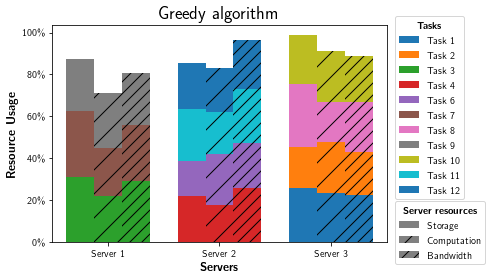
\includegraphics[width=\linewidth]{figs/allocation/greedy_algorithm.png}
    \caption{Example Greedy allocation using the model from table~\ref{tab:example-tasks-properties}
    and~\ref{tab:example-servers-properties}}
    \label{fig:greedy-allocation}
\end{figure}

\begin{algorithm}
    \caption{Pseudo code of Greedy Mechanism}
    \label{alg:greedy-mechanism}
    \begin{algorithmic}
        \REQUIRE $J$ is the set of tasks and $I$ is the set of servers
        \REQUIRE $S^{'}_i$, $W^{'}_i$ and $R^{'}_i$ is the available resources (storage, computation and bandwidth respectively) of server $i$
        \REQUIRE $\alpha(j)$ is the value density function of task $j$
        \REQUIRE $\beta(j, I)$ is the server selection function of task $j$ and set of servers $I$ returning the best server, or $\emptyset$ if the task is not able to be run on any server
        \REQUIRE $\gamma(j, i)$ is the resource allocation function of a task and server returning the loading, compute and sending speeds
        \REQUIRE $\text{sort}(X, f)$ is a function that returns a sorted list of elements in descending order, based on a set of elements $X$ and a function for comparing elements $f$

        \STATE{$J^{'} \leftarrow sort(J, \alpha)$}
        \FORALL{$j \in J^{'}$}
        \STATE{$i \leftarrow \beta(j, I)$}
        \IF{$i \neq \emptyset$}
        \STATE{$s^{'}_j, w^{'}_j, r^{'}_j \leftarrow \gamma(j, i)$}
        \STATE{$x_{i,j} \leftarrow 1$}
        \ENDIF
        \ENDFOR
    \end{algorithmic}
\end{algorithm}

Using the greedy mechanism (algorithm~\ref{alg:greedy-mechanism}), the time complexity is polynomial,
$O(\left|J\right| \left|I\right|)$.
\begin{theorem}
    Time complexity of the greedy mechanism is $O(\left|J\right| \left|I\right|)$, where $\left|J\right|$ is the number
    of tasks and $\left|I\right|$ is the number of servers. Assuming that the value density and resource allocation
    heuristics have constant time complexity and the server selection function is $O(\left|I\right|)$.
    %% TODO to check if the resource allocation heuristic is constant time complexity (KKT) probably wrong
\end{theorem}
\begin{proof}
    The time complexity of the stage 1 of the mechanism is $O(\left|J\right| \log(\left|J\right|))$ due to sorting the
    tasks and stage 2 has complexity $O(\left|J\right| \left|I\right|)$ due to looping over all of the tasks and
    applying the server selection and resource allocation heuristics. Therefore the overall time complexity is
    $O(\left|J\right| \left|I\right| + \left|J\right| \log(\left|J\right|) = O(\left|J\right| \left|I\right|)$.
\end{proof}

\subsection{Critical Value Auction}\label{subsec:critical-value-auction}
Due to the problem case being non-cooperative, if the greedy mechanism was used to allocate resources such that the
value is the price paid. This would be open to manipulation and misreporting of task attributes like the value,
deadline or resource requirements. Therefore in this section we propose an auction that is strategyproof
(weakly-dominant incentive compatible) so users have no incentive to misreport task attributes.

Single-Parameter domain auctions are extensively studied in mechanism design~\cite{nisan2007algorithmic_228} and are
used where an agent's valuation function can be represented as single value. The task price is calculated by finding
the critical value, the minimum task price required for the task to still allocated by the greedy mechanism. This has
been shown to be a strategyproof~\cite{nisan2007algorithmic_229_230} auction making it a weakly-dominant strategy for
a user to honestly reveal a task's attribute.

The auction is implemented using the greedy mechanism from section~\ref{subsec:greedy-mechanism} to find an allocation
of tasks using the reported value. The critical value for each task is found by rearranging the value density function
to makes the value the subject and the value density of the task equal to the minimum value density such the task is
still allocated in the list. Because of this, the time complexity is the same as the greedy mechanism,
$O(\left|J\right| \log(\left|J\right|))$ as it is just repeating this mechanism twice. The first to find the tasks
allocated normally with the second allocation, running through all of the tasks allocated to check the last position
in the value density list to find the position where the task couldn't be allocated on any server.

In order that the auction is strategyproof, the value density function must be
monotonic~\cite{nisan2007algorithmic_229_230} so that misreporting of any task attributes will result in the value
density decreasing. Therefore a value density function of the form $\frac{v_j d_j}{\alpha(s_j, w_j, r_j)}$ must be used so
that the auction is strategyproof.
\begin{theorem}
    The value density function $\frac{v_j d_j}{\alpha(s_j, w_j, r_j)}$ is monotonic increasing for task $j$ assuming the
    function $\alpha(s_j, w_j, r_j)$ is monotonic increasing.
\end{theorem}
\begin{proof}
    In order to misreport the task value and deadline, misreported values must be less than their true value, therefore
    if the value or deadline are decreased then the density will likewise decrease.
    While the opposite is true for the required resources (storage, compute and result data) as the misreported value
    must be greater than the true value. As the $\alpha$ function is will increase as the resource requirements increase,
    the resulting density will decrease.
\end{proof}

\subsection{Decentralised Iterative Auction}\label{subsec:decentralised-iterative-auction}
In some application of edge cloud computing, keeping the value of a task a secret is important for example
military-tactical networks. Therefore we propose a novel decentralised iterative auction based on the pricing principle
of the VCG auction~\cite{vickrey,Clarke,groves}. VCG auctions calculates the price of a tasks by finding the
difference in social welfare if the task is considered in the allocation and when the task isn't. Our proposed novel
auction uses the same principle, except without requiring a task value, by calculating a task's price by finding the
difference between the current server revenue and the revenue when the task is required to be allocated with zero value.

Our auction uses this principle by iteratively letting a task advertise its requirements to all of the servers, who
respond with their price to run the task. This price is equal to the server's current revenue minus the solution to the
problem in section~\ref{subsubsec:decentralised-iterative-problem} plus a small value referred to as the price change
variable. The reason for the price change variable is to increase the revenue of the server (otherwise the total
revenue of the server doesn't increase by accepting the task) and is be chosen by the server. Once all of the servers
have responded, the task can compare the minimum server prices to its private value. If the price is less then the
task will accept the server with the lowest price, otherwise the task must stop advertising as the price for the task
to run on any server is greater than its reserve price preventing the task from ever being allocated again.

\subsubsection{Server revenue optimisation problem}\label{subsubsec:decentralised-iterative-problem}
To find the optimal revenue for a server $m$ given a new task $n^{'}$ and set of currently allocated tasks $N$ has a
similar formulation to the optimisation problem in section~\ref{subsec:optimisation-problem}. Except with an additional
variable for the task price $p_n$ for each task $n$.

\begin{align}
    \max & \sum_{\forall n \in N} p_n x_n\label{eq:dia-objective}\\
    \mbox{s.t.} \nonumber \\
    & \sum_{\forall n \in N} s_n x_n + s_{n^{'}} \leq S_m,\label{eq:dia-server-storage-constraint}\\
    & \sum_{\forall n \in N} w^{'}_n x_n + w_{n^{'}} \leq W_m, \label{eq:dia-server-computation-constraint}\\
    & \sum_{\forall n \in N} (r^{'}_n + s^{'}_n) \cdot x_n + (r^{'}_{n^{'}} + s^{'}_{n^{'}}) \leq R_m, \label{eq:dia-server-communication-constraint}\\
    & \frac{s_n}{s^{'}_n} + \frac{w_n}{w^{'}_n} + \frac{r_n}{r^{'}_n} \leq d_n, &~ \forall n \in N \cup \{n^{'}\} \label{eq:dia-task-deadline}\\
    & 0 < s^{'}_n < \infty, &~ \forall{n \in N \cup \{n^{'}\}} \label{eq:dia-loading-speeds}\\
    & 0 < w^{'}_n < \infty, &~ \forall{n \in N \cup \{n^{'}\}} \label{eq:dia-compute-speeds}\\
    & 0 < r^{'}_n < \infty, &~ \forall{n \in N \cup \{n^{'}\}} \label{eq:dia-sending-speeds}\\
    & x_n \in \{0,1\} &~ \forall{n \in N} \label{eq:dia-job-allocation}
\end{align}

The objective (Eq.~\eqref{eq:dia-objective}) is to maximize the price of all currently allocated tasks (not including
the new task as the price is zero). The server resource capacity constraints
(Eqs.~\eqref{eq:dia-server-storage-constraint},~\eqref{eq:dia-server-computation-constraint}
and~\eqref{eq:dia-server-communication-constraint}) are similar to the constraints in the standard model set out in
section~\ref{subsec:optimisation-problem} except with the assumption that the task $n^{'}$ is running so there is no
need to consider if it is running or not. The deadline and non-negative resource speeds constraints
(\ref{eq:dia-task-deadline},~\ref{eq:dia-loading-speeds},~\ref{eq:dia-compute-speeds} and~\ref{eq:dia-sending-speeds})
are all the same equation as the standard formulation for all of the tasks plus the new task. As this formulation only
considers a single server, the task allocation constraint is not consider.

For our proposed auction, we consider four important properties in auction theory.
\begin{itemize}
    \item Budget balanced - True, since the auction can run without an auctioneer, the auction can be run in a
    decentralised system resulting in no ''middlemen'' taking some money meaning that all revenue goes straight to
    the servers from the tasks.
    \item Individually Rational - True, as the server need to confirm with the task if it is willing to pay an amount
    to be allocated, the task can check this against its secret reserved price preventing the task from ever paying
    more than it is willing.
    \item Incentive Compatible - False, as major problem for tasks is being deallocated from a server. Task can
    misreport its attribute making it cheaper for another task to be allocated to another server preventing the
    misreported task from being deallocated.
    \item Economic efficiency - False, at the beginning tasks are almost randomly assigned till servers become full and
    require kicking tasks off. This can cause the allocation to fall into a local price maxima meaning that the
    server will sometimes not be 100\% economically efficient.
\end{itemize}

The algorithm~\ref{alg:dia} is a centralised version of the auction. It works through iteratively checking a currently
unallocated job to find the price if the job was currently allocated on a server. This is done through first solving
the program in section~\ref{subsubsec:decentralised-iterative-problem} which calculates the new revenue if the task was
forced to be allocated with a price of zero. The task price is equal to the current server revenue minus the new
revenue with the task allocated plus a price change variable in order to increase the revenue of the server. The
minimum price returned by $P(i, k)$ is then compared to the job's maximum reserve price (that would be private in the
equivalent decentralised algorithm) to confirm if the job is willing to pay at that price. If the job is willing then
the job is allocated to the minimum price server and the job price set to the agreed price. However in the process of
allocating a job then the currently allocated jobs on the server could be unallocated so these jobs allocation's and
price's are reset then appended to the set of unallocated jobs.

\begin{algorithm}[H]
    \caption{Decentralised Iterative Auction}
    \label{alg:dia}
    \begin{algorithmic}
        \REQUIRE $I$ is the set of servers
        \REQUIRE $J$ is the set of unallocated tasks, which initial is the set of all tasks to be allocated
        \REQUIRE $P(i, k)$ is solution to the problem in section~\ref{subsubsec:decentralised-iterative-problem}
        using the server $i$ and new task $k$.
        The server's current tasks is known to itself and its current revenue from tasks so not passed as arguments.
        \REQUIRE $R(i, k)$ is a function returning the list of tasks not able to run if task $k$ is allocated to server $i$
        \REQUIRE $\leftarrow_R$ will randomly select an element from a set
        \WHILE{$|J| > 0$}
        \STATE{$j \leftarrow_R J$}
        \STATE{$p, i \leftarrow argmin_{i \in I} P(i, j)$}
        \IF{$p \leq v_j$}
        \STATE{$p_j \leftarrow p$}
        \STATE{$x_{i, j} \leftarrow 1$}
        \FORALL{$j^{'} \in R(i, j)$}
        \STATE{$x_{i, j^{'}} \leftarrow 0$}
        \STATE{$p_j^{'} \leftarrow 0$}
        \STATE{$J \leftarrow J \cup j^{'}$}
        \ENDFOR
        \ENDIF
        \STATE{$J \leftarrow J \setminus \{j\}$}
        \ENDWHILE
    \end{algorithmic}
\end{algorithm}

\subsection{Attributes of proposed algorithms}\label{subsec:attributes-of-proposed-algorithms}
In this paper, we have presented three mechanisms to solve the optimisation problem proposed in
section~\ref{subsec:optimisation-problem}. The table~\ref{tab:attributes_algorithms} considers a range of
important attributes of the proposed algorithm to allow easy comparison between the Greedy mechanism (GM),
Critical Value auction(CVA) and Decentralised Iterative auction (DIA).

\begin{table}[H]
    \centering
    \begin{tabular}{|p{2.2cm}|p{1.5cm}|p{1.5cm}|p{1.5cm}|}
        \hline
        Attribute                           & GM  & CVA & DIA                   \\ \hline
        Truthfulness                        &     & Yes & No                    \\ \hline
        Optimality                          & No  & No  & No                    \\ \hline
        Scalability                         & Yes & Yes & No                    \\ \hline
        Information requirements from users & All & All & Not the reserve value \\ \hline
        Communication over heads            & Low & Low & High                  \\ \hline
        Decentralisation                    & No  & No  & Yes                   \\ \hline
    \end{tabular}
    \caption{Attributes of the proposed algorithms: Greedy mechanism (GM), Critical Value auction(CVA) and Decentralised Iterative auction (DIA)}
    \label{tab:attributes_algorithms}
\end{table}

    \section{Empirical Evaluation}\label{sec:empirical-evaluation}
To test the algorithms presented in section~\ref{sec:flexible-resource-allocation-mechanisms}, synthetic models have
been used to generate a list of tasks and servers. These models have been handcrafted with each attribute being
generated from a Gaussian distribution with a mean and standard deviation.

To compare the greedy algorithm to the optimal elastic allocation, a branch and bound was implemented to solve the
optimisation problem in section~\ref{subsec:optimisation-problem}. In order to compare to fixed speed equivalent models,
the minimum total resource required to run the job is found and set as the resource speeds for all of the tasks, with
the optimal solution for running the job with the fixed speeds is found as well. To implement the greedy mechanism, the
value density function was $\frac{v_j}{s_j + w_j + r_j}$, server selection was
$\text{argmin}_{\forall i \in I} S^{'}_i + W^{'}_i + R^{'}_i$ and the resource allocation was
$\text{min} s^{'}_j + w^{'}_j + r^{'}_j$ for job $j$ and servers $I$.

% Greedy mechanisms
\begin{figure}[h]
    \centering
    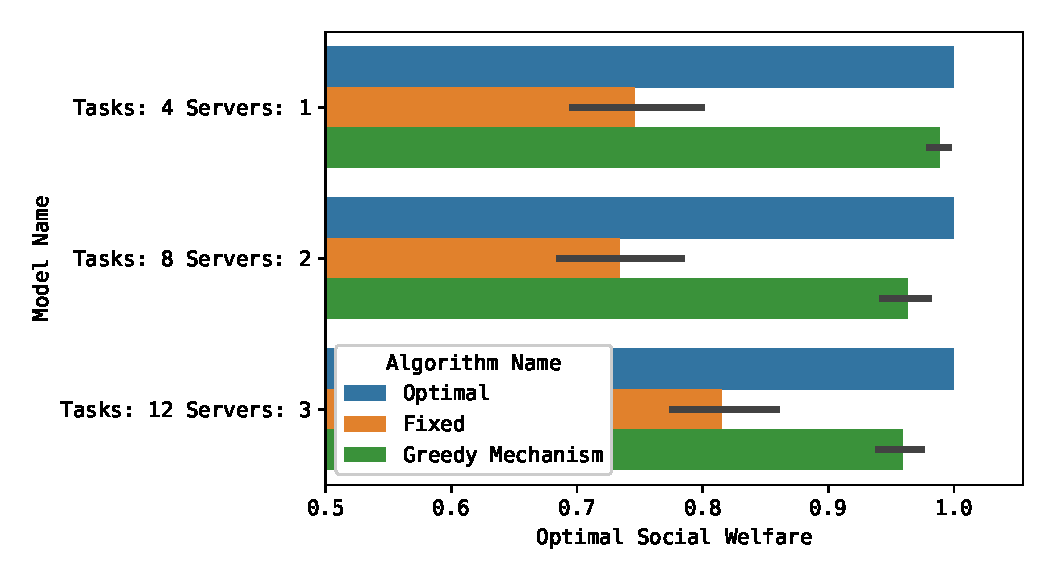
\includegraphics[width=\linewidth]{fig/empirical_evidence/greedy_mechanism.eps}
    \caption{Comparison of the social welfare for the greedy mechanism, optimal, relaxed problem, time limited branch and bound}
    \label{fig:greedy_mechanism_comparison}
\end{figure}
As figure~\ref{fig:greedy_mechanism_comparison} shows, the greedy mechanism achieves 98\% of the optimal solution for
the small models, the mechanism achieves within 95\% for larger models. In comparison, the fixed allocation achieves
80\% of the optimal solution and always does worse than the social welfare of the greedy mechanism.

% Auction mechanisms
\begin{figure}[h]
    \centering
    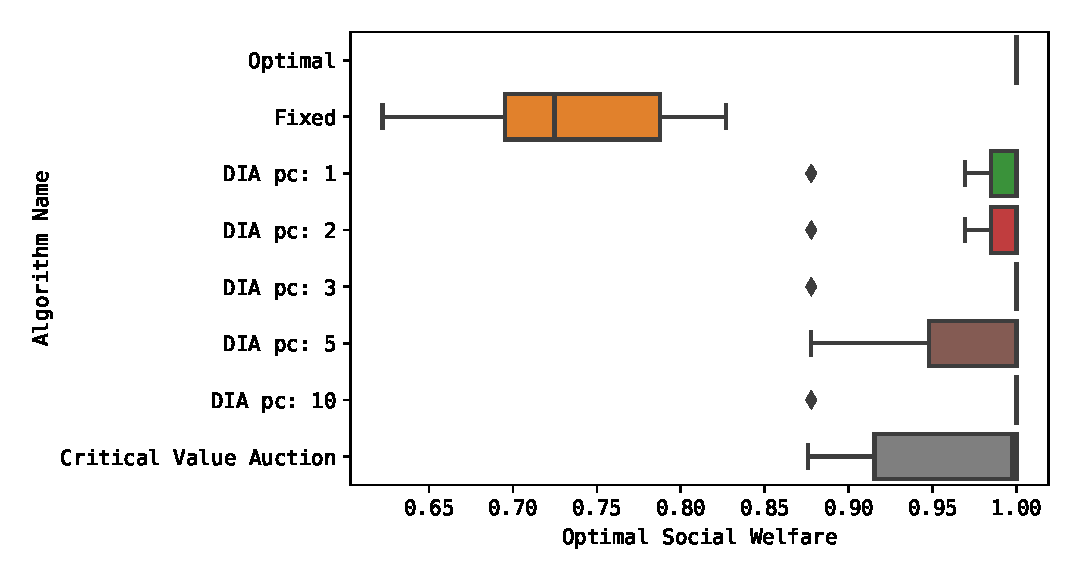
\includegraphics[width=\linewidth]{fig/empirical_evidence/auction_mechanisms.eps}
    \caption{Comparison of the social welfare for the auction mechanisms}
    \label{fig:auction_mechanisms_comparison}
\end{figure}
Figure~\ref{fig:auction_mechanisms_comparison} compares the social welfare of the auction mechanisms: VCG auction,
fixed resource speed VCG auction, critical value auction and the decentralised iterative auction with different price
change variables.

% Round number
\begin{figure}[h]
    \centering
    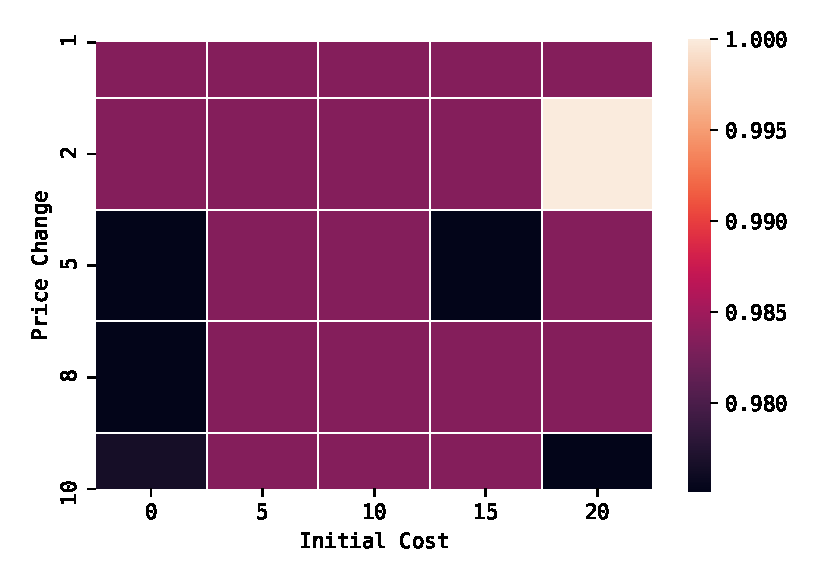
\includegraphics[width=\linewidth]{fig/empirical_evidence/iterative_round_number.eps}
    \caption{Average number of rounds with a price change variables and task initial cost}
    \label{fig:iterative_round_number}
\end{figure}
\begin{figure}[h]
    \centering
    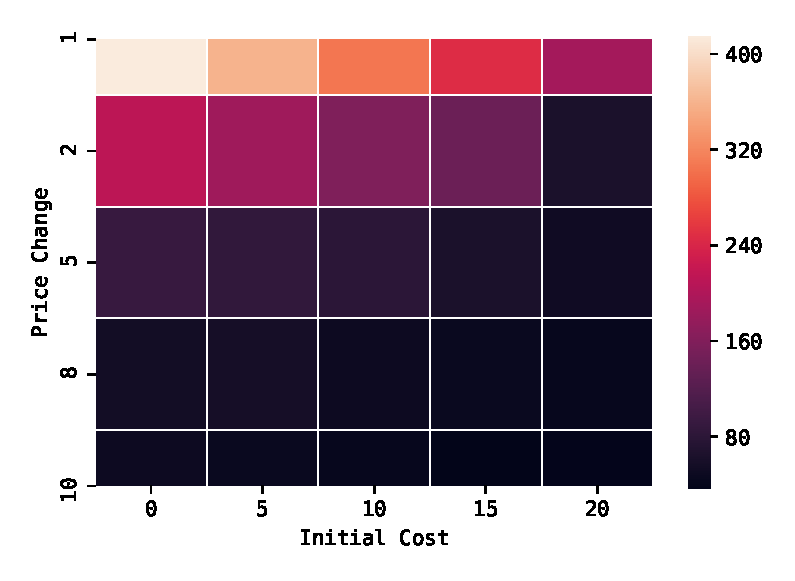
\includegraphics[width=\linewidth]{fig/empirical_evidence/iterative_social_welfare.eps}
    \caption{Average social welfare with a price change variables and task initial cost}
    \label{fig:iterative_social_welfare}
\end{figure}
Within the context of edge cloud computing, the number of rounds for the decentralised iterative auction is important
to making it a feasible auction as it is proportional to the time required to run. We investigated the effect of two
heuristic on the number of rounds and social welfare of the auction; the price change variable and initial cost
heuristic. With an auction using as minimum heuristic values for the price change and initial cost,
figure~\ref{fig:iterative_round_number}, on average 400 rounds were required for the price to converge while an auction
using a price change of 10 and initial cost of 20 means that only on average 80 rounds are required, 5x less. But by
using high initial cost and price change heuristics, this can prevent tasks from being allocated,
figure~\ref{fig:iterative_social_welfare}, shows that the difference in social welfare is only 2\% from minimum to
maximum heuristics.

% Mutation auction
% \begin{figure}
%    \centering
%    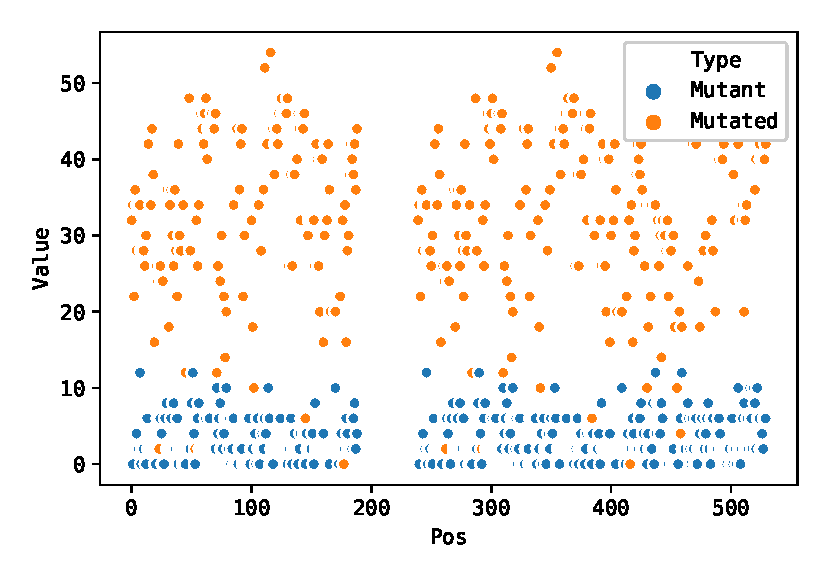
\includegraphics[width=\linewidth]{empirical_evidence_figures/mutate_auction.eps}
%    \caption{Difference in task price to a truthful task and misreported task}
%    \label{fig:auction_mutation}
%\end{figure}
%As the decentralised iterative auction presented in section \ref{subsec:decentralised-iterative-auction} is not
%incentive compatible, it is possible that misreporting of task attribute can decrease the price paid by a task.
%Figure \ref{fig:auction_mutation} is a scatter graph of the  a task (in orange) and the price of a misreported task
%(in blue). Misreported task were generated by increase the task resource requirements or by decreasing the task value
%or deadline that would substituted for the original truthful task. As the figure clearly shows, in almost all cases of
%mutation causes the


\section{Conclusions}\label{sec:conclusions-and-future-work}
In this paper, we studied a resource allocation problem in edge clouds, where resources are elastic and can be
allocated to tasks at varying speeds to satisfy heterogeneous requirements and deadlines. To solve the problem,
we proposed a centralized greedy mechanism with a guaranteed performance bound, and a number of auction-based
mechanisms that also consider the elasticity of resources and limit the potential for strategic manipulation. We show
that explicitly taking advantage of resource elasticity leads to significantly better performance than current
approaches that assume fixed resources.

In future work, we plan to consider the dynamic scenario where tasks arrive and depart from the system over time, and
to also consider the case where task preemption is allowed.

%%%%%%%%%%%%%%%%%%%%%%%%%%%%%%%%%%%%%%%%%%%%%%%%%%%%%%%%%%%%%%%%%%%%%%%%%%%%%%%%%%%%%%%%%%%%%%%%%%%%%%%%%
    %% bibliography: see CFP for number of permitted pages
    \balance
    \bibliographystyle{ACM-Reference-Format}  % do not change this line!
    \bibliography{bibliography}  % put name of your .bib file here

\end{document}